\documentclass[12pt]{article}%
\usepackage{xdipp}
% \pismo{Constantia} % nic (=LModern), Academia, Bookman, Cambria, Constantia, Palatino, Times % not available on overleaf
\popiskyzkr % \popisky % implicitní
\pagestyle{headings} % implicitní
\cislovat{2}
\brokenpenalty 10000

% my additional packages start here:
\usepackage{hyperref}

\begin{document}
%\tracingall % additional error messages
\titul{Plánování výsledku hospodaření pro podnik  	Mlékárna Valašské Meziříčí, spol. s. r.o.}{}{Tomáš Hanzely\\Josef Sysel\\Lukáš Janoušek}{Brno 2019}

\obsah
\newpage\listoffigures
\newpage\listoftables


\kapitola{Uzitecne linky}
ICO: 46578323 \\ 
\url{https://www.mlekarna-valmez.cz/}
\\\\
\href{https://or.justice.cz/ias/ui/vypis-sl-detail?dokument=54352087&subjektId=214813&spis=823166}{účetní závěrka: 2017} \\
\href{https://or.justice.cz/ias/ui/vypis-sl-detail?dokument=45266633&subjektId=214813&spis=823166}{účetní závěrka: 2016} \\ 
\href{https://or.justice.cz/ias/ui/vypis-sl-detail?dokument=45266633&subjektId=214813&spis=823166}{účetní závěrka: 2015} \\ 
\href{https://or.justice.cz/ias/ui/vypis-sl-detail?dokument=40394224&subjektId=214813&spis=823166}{účetní závěrka: 2014} \\ 
\href{https://or.justice.cz/ias/ui/vypis-sl-detail?dokument=17927050&subjektId=214813&spis=823166}{účetní závěrka: 2013} \\ 
\href{https://or.justice.cz/ias/ui/vypis-sl-detail?dokument=17277179&subjektId=214813&spis=823166}{účetní závěrka: 2012} \\ 
\\
\href{https://www.merk.cz/search/detail/cz-46578323/?fbclid=IwAR0feartZTdMqdPtmH1MulFQq-QUbhAvphTyT_J-R3s8eGWLKt2KoLLMt7Q#tab_overview}{2010-2016 (overview)} \\


%%%%%%%%%%%%%%%%%%%%%%%%%%%%%%%%%%%%%%
%%%%%%%%%%%%%%%%%%%%%%%%%%%%%%%%%%%%%%

\kapitola{Úvod} (Lukas)
todo

\sekce{Cíl práce} (Lukas)
todo


\kapitola{Analýza vnějšího prostředí}

\sekce{PEST(Hanzely)}
\subsubsection*{Ekonomické prostředí}
Predpokladom zvyšovanie výkonnosti ekonomiky je rast HDP. Výkonnosť ekonomiky tak odzrkadľuje celkovú spotrebu v spoločnosti. Vyššia spotreba teda predpokladá aj vyššiu produkciu, ktorá sa dotýka podnikov priamo. Za posledných 10 rokov je HDP Českej republiky medziročne rastúce. Poľnohospotárstvo tvorí 2.2\% celkovej produkcie. Keďže je ale mlieko nezbytný tovar, domácnosti budú mlieko kupovať nezávisle na výške HDP, alebo ekonomickom cykle. Vyššia kúpna sila však do určitej miery zvýši predaje mlieka, až na určitú úroveň, kde domácnosť nebude schopná spotrebovať toľko mlieka. Zvýšená kúpna sila však podporí spotrebu iných mliečnych výrobkov, ktoré sa nepokladajú za nevyhnutné. Taktiež bude mať za následok zvýšenie spotreby iných protuktov súvisiacich so spotrebou mlieka ako napríklad zakúpenie domáceho zvieraťa. Kúpnu silu tiež ovplyvňuje úroveň inflácie alebo nezamestnanosti. V roku 2017 stúpla inflácia na úroveň 2.5\% a v roku 2018 bola na úrovni 2.1\%, kdežto v rokoch 2014 až 2016 sa držala na úrovni pod 1\%, to bolo spůsobené prudším rastom cien. Úroveň nezamestananosti ma za posledných 5 rokov klesavú tendenciu, kde v roku 2013 bola na úrovni 8.2\% dnes dosahuje úroveň  3.1\%, čo pozitívne ovplyvňuje kúpnu silu. Vývoj reálnej mzdy má tiež stúpavý trend, kde za posledných 5 rokov bol nárast o 5.8\%. 

\subsubsection*{Socialní prostředí}
Moderný životný štýl, kde stále viac ľudí dbá o zdravú výživu a strach s obezity so všeobecným presvedšením, že plnotučné výrobky k tomu možu dopomosť znižuje predajnosť plnotučných mliečnych výrobkov. Tendencia zákazníkov je teda prejsť na nízkotučné, prípadne odtučnené varianty tomu by sa mala prisposobiť aj ponuka producentov. 
V poslednej dobe moderný vegánsky štýl stravovania zase negatívne ovplyvňuje predaje mliečnych výrobkov, kedže ich životný štýl nepovoľuje konzumáciu akých koľvek mliečnych výrobkov so živočišného mlieka. Na lokalnom trhu nie veľmi rozsiahly problém predstavuje halal, to predstavuje určité obmedzenia kladené na produkt spojené so sposobom získania tohoto produktu. Moslimovia konzumujú len také mliečne výrobky, ktoré veria že sú v súlade s týmito pravidlami a sú halal. 
\subsubsection*{Technologicé a technické prostředí}

\subsubsection*{Politicko-právní prostředí}
Legistaívne má veľký vplyv na trh mlieka a mliečnych výrobkov Európska únia a ňou vedelná spoločná poľnohospodárska politika. Toto odvetvie je na rozdiel od iných odvetví, ktoré sú predmetom vnútroštátnych politík, výhradne podporované na európskej úrovni. Jej cieľom je stanovovať spoločné ciele, zásady a pravidlá cím garantuje spravodlivé podmienky. Za rok 2011 predstavovala táto politika 43\% európskeho rozpočtu, čo predstavuje približne 30 centov na občana EÚ denne.%(http://europa.eu/rapid/press-release_MEMO-13-631_sk.htm). Z pohľadu českej legistatívy sú důležité hlavne dva zákony a to:
\begin{itemize}
	\item Zákon č. 110/1997 Sb., vplatném znění, tzv. „Zákon o potravinách“ - účelom tohoto zákona je stanoviť dozor nad dodržovaním povnností potravinárskych podnikov v súlade s právom EÚ %[ČR. Sbírka zákonů 1997 ČESKÉ REPUBLIKY číslo 110/1997  Sb.,Zákono  potravi-nách, a tabákových výrobcích a doplnění některých souvisejících zákonů. Částka 38. Do-stupný také z: hthttp://aplikace.mvcr.cz/sbirkazakonu]
	\item Zákon č. 166/1997 Sb., vplatném znění, tzv. „Veterinární zákon“ %[ČR. Sbírka zákonů 1997 ČESKÉ REPUBLIKY číslo 110/1997  Sb.,Zákono  potravi-nách, a tabákových výrobcích a doplnění některých souvisejících zákonů. Částka 38. Do-stupný také z: hthttp://aplikace.mvcr.cz/sbirkazakonu]
	\item Nařízení Evropského parlamentu a Rady (ES) č. 852/2004 - nariadenie sa zaoberá správnou hygienou potravín, a stanovuje zodpovednosť práve prevádzkovateľom potravinárskych podnikov %[http://www.khsova.cz/docs/01_legislativa/files/852_2004.pdf]
	\item Nařízení Evropského parlamentu a Rady (ES) č. 853/2004 - presnešia špecifikácia hygieny, materiálov a kvalitatívnych parametrov prístrojov, pracovníkov a práce s potravinami. %[http://www.khsjih.cz/soubory/predpisy-eu/narizeni-eu-853.pdf]
\end{itemize}

\subsection{Porterov model 5F} (Lukas)
todo

\subsection{McKinsey 7S} (Lukas)
todo

\sekce{SWOT} (Josef)
SWOT analýzou se pokusíme zanalyzovat tvář naší firmy po stránce vnitřního a vnějšího prostředí.


\subsection*{Vnitřní prostředí podniku}

\subsection*{Vnější prostředí podniku}

\subsection*{}

\subsection*{}

\subsection*{}

\subsection*{}

- silne / slabe stranky ...vnejsi prostredi
- naklady nase vs konkurence
- hrozby a prilezitosti

\sekce{Finanční analýza}
todo

\subsection{Analýza absolutních ukazatelů} (Lukas)
todo

\subsection{Analýza rozdílových ukazatelů} (Josef)
todo
- cash flow


\subsection{Analýza poměrových ukazatelů(Hanzely)}
\subsubsection*{Likvidita}
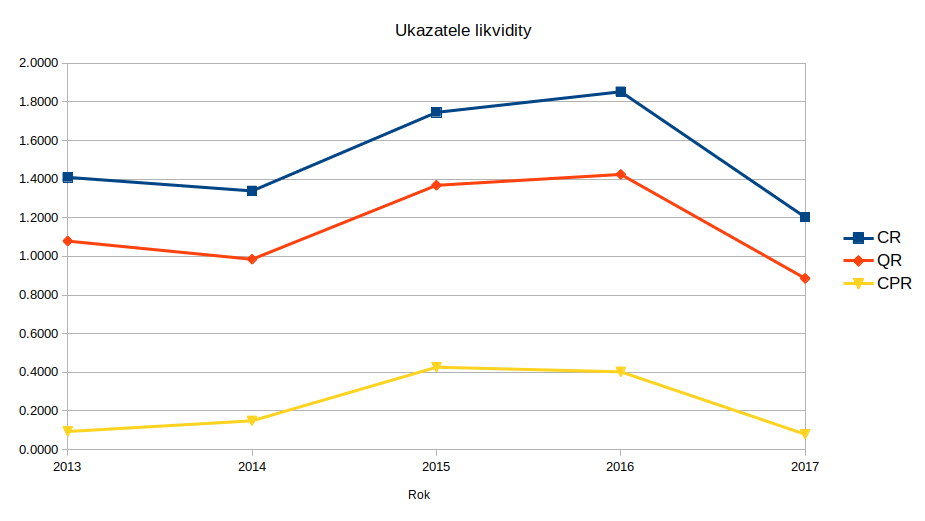
\includegraphics[scale=0.6]{obr/ukazatele_likvidity.png}
\subsubsection*{Rentabilita}
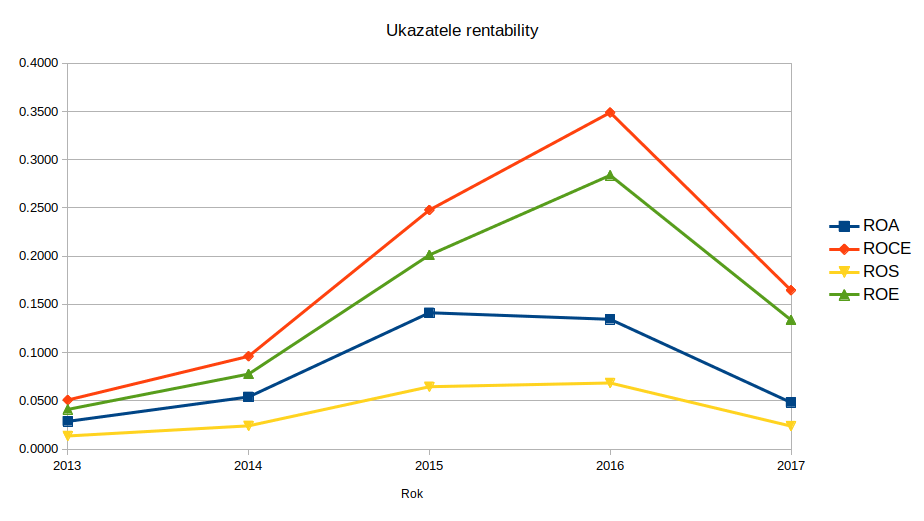
\includegraphics[scale=0.6]{obr/ukazatele_rentability.png}
\subsubsection*{Zadluženost}
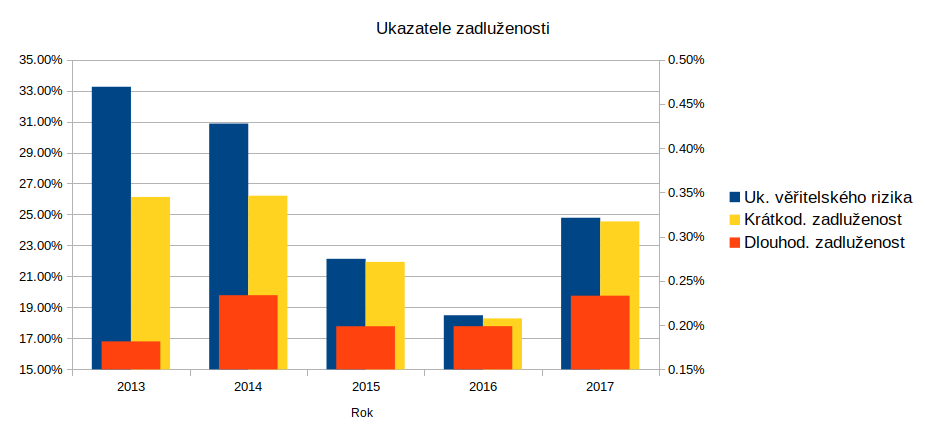
\includegraphics[scale=0.6]{obr/ukazatele_zadlzenosti1.png} \\
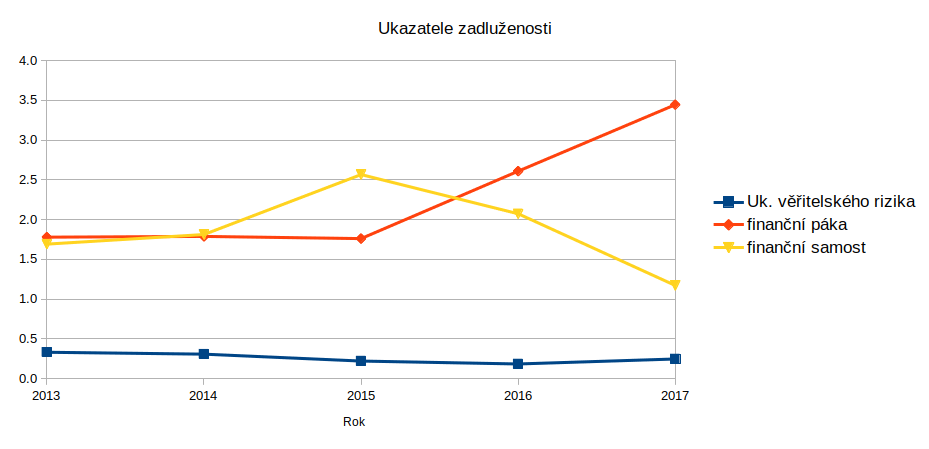
\includegraphics[scale=0.6]{obr/ukazatele_zadlzenosti.png}
\subsubsection*{Aktivita}
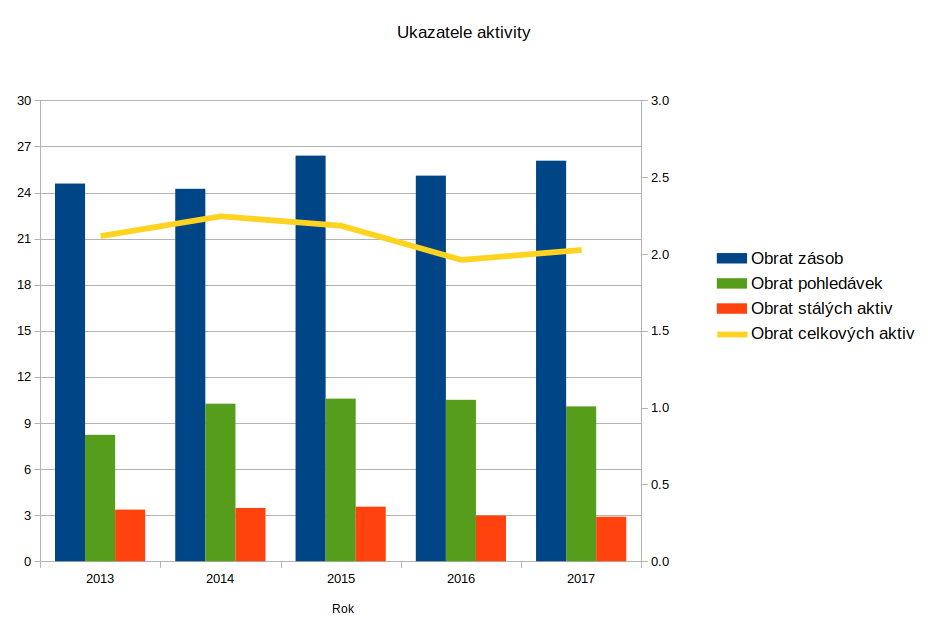
\includegraphics[scale=0.6]{obr/ukazatele_aktivity.png} \\
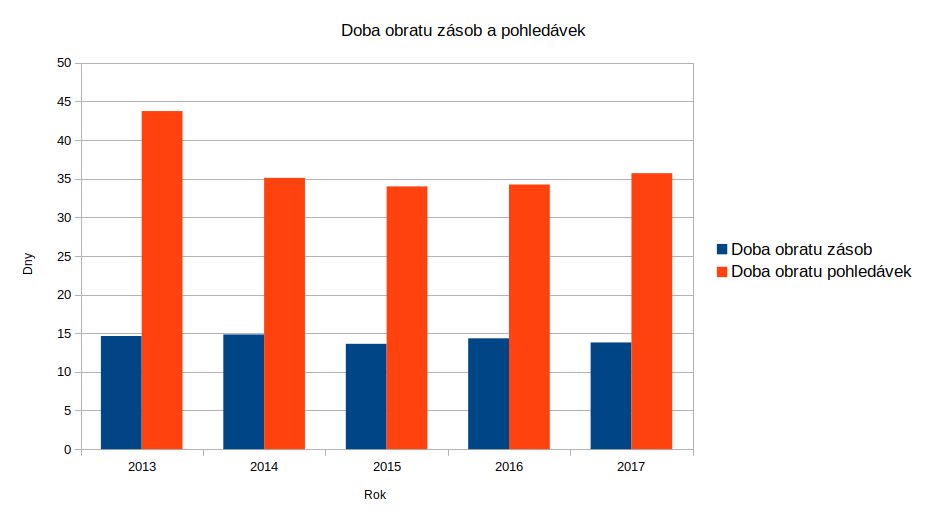
\includegraphics[scale=0.6]{obr/doba_obratu.png}




\kapitola{Závěr}
todo

%%%%%%%%%%%%%%%%%%%%%%%%%%%%%%%%%%%%%%
%%%%%%%%%%%%%%%%%%%%%%%%%%%%%%%%%%%%%%

\kapitola{Tipy a Triky}
%----------------- příkazy pro sazbu příkazů
\def\bsl{\char92}
\def\lsv{\char123}
\def\rsv{\char125}
%----------------- konec mezidefinic


\sekce{Příprava vlastního textu}


\tabulka{Sazba speciálních znaků v~hladkém textu}

\label{speczn}
\def\arraystretch{1.2}
\footnotesize
\tabcolsep 2.5pt
\begin{tabular}{|p{.16\textwidth}|p{.48\textwidth}|l|l|} \hline
\textbf{Znak} & \textbf{Zápis v~textu} & \textbf{Příklad} & {\bfseries
Vysázeno} \\ \hline\hline
Mezera & Stisk mezerníku (i~několikanásobný) & & \\ \hline
Nezlomitelná\newline mezera & \texttt{\char126} (ručně nebo spuštěním
programu pro \newline automatické vložení za předložky) &
\texttt{u\char126okna} & u~okna\\ \hline
%Zúžená mezera 1/4 em & \texttt{\bsl,} & \texttt{P.\bsl,Král} & P.\,Král\\ \hline
%Zúžená mezera 1/6 em & \texttt{\bsl;} -- používá se k~mezerování výpustky & 
         \texttt{přišel\bsl;\bsl dots} & přišel\;\dots\\ \hline
Široká mezera & \texttt{\bsl quad} (čtverčík -- 1 em) \texttt{\bsl qquad} (2
em) & \texttt{$a=b$\bsl quad $b=c$} & $a=b$\quad $b=c$\\ \hline
Odstavec & Vynechaný řádek (i~vícenásobně) & &\\ \hline
Tři tečky & \texttt{...} nebo \texttt{\bsl dots} & \texttt{zanikl\bsl;\bsl
dots} & zanikl\;\dots \\
\hline
Spojovník & \texttt{-} (přímo z~klávesnice) & \texttt{bude-li} & bude-li \\ \hline
Spojovník & \texttt{\bsl spoj} (tento spojovník se při řádkovém zlomu\newline
přetahuje na začátek následujícího řádku) & \texttt{bude\bsl spoj\lsv\rsv li} &
\polet l{bude-\\-li} \\ \hline
Pomlčka & \texttt{-{}-} (půlčtverčíková) \texttt{-{}-{}-} (čtverčíková) &
\texttt{6-{}-12} & 6--12 \\ \hline
Pomlčka \newline (rozsahová) & \texttt{\bsl az} (tato pomlčka se při řádkovém
\newline zlomu nahradí slovem \uv{až})  & \texttt{6\bsl az 12}& 6--12, \polet
r{nebo 6\\až 12} \\ \hline
Znak minus & \texttt{\char36-\char36} (v~matematickém režimu) &
\texttt{\char36-10\char36} & $-10$ \\ \hline
Znak násobení & \texttt{\char36\bsl times\char36} nebo přímo z~klávesnice × & \texttt{\char36 2\bsl
times 3\char36\bsl,mm} & $2\times 3$\,mm\\ \hline
Stupeň & \texttt{\char36\char94\bsl circ\char36} &
\texttt{5\bsl,\char36\char94\bsl circ\char36C} & 5\,$^{\circ}$C \\ \hline
Paragraf & (jen s~číslem) \texttt{\bsl S} nebo přímo z~klávesnice §  & \texttt{\bsl S\bsl,36}& \S\,36 \\ \hline
Značky \newline \#, \$ a~\& & \texttt{\bsl\#}, \texttt{\bsl\char36},
\texttt{\bsl\&} & & \\ \hline
Závorky \{ a~\} & \texttt{\bsl\lsv}, \texttt{\bsl\rsv} & &\\ \hline
Značky $<$ a~$>$ & \texttt{\char36\char60\char36}, \texttt{\char36\char62\char36}
& \texttt{\char36a\char62 b\char36} & $a>b$\\ \hline
Procento & \texttt{\bsl\char37} & \texttt{10\bsl,\bsl\char37}& 10\,\% \\ \hline
Uvozovky & \texttt{\bsl uv\lsv}text\texttt{\rsv} & \texttt{\bsl uv\lsv
Něco\rsv} & \uv{Něco}\\ \hline
Uvozovky \newline (úhlové) & \texttt{\bsl uvv\lsv}text\texttt{\rsv} &
\texttt{\bsl uvv\lsv Něco\rsv} & \uvv{Něco}\\ \hline
\end{tabular}
\endtab

V~textu lze používat příkazy pro vyznačení -- základní vyznačení
\verb.\emph{text}., pro důležité pojmy pak tučného řezu příkazem
\verb.\textbf{text}., kapitálky jsou dostupné příkazem \verb.\textsc{text}..


\begin{literatura}
\citace{beran}{Beran, 1994}{\autor{Beran, V.} \nazev{Typografický manuál.}
Náchod: Nakladatelství Manuál, 1994. \\ ISBN 80-901824-0-2}

\citace{csn010166}{ČSN 01\,0166, 1992}{\nazev{ČSN 01\,0166 Nakladatelská
(vydavatelská) úprava knih a~některých dalších druhů neperiodických
publikací.} Praha: Federální úřad pro normalizaci a~měření, 1992}

\citace{csn016910}{ČSN 01\,6910, 2014}{\nazev{ČSN 01\,6910 Úprava dokumentů
zpracovaných textovými procesory.} Praha: ÚNMZ, 2014}

\citace{csniso690}{ČSN ISO 690, 2011}{\nazev{ČSN ISO 690 -- Bibliografické
citace. Obsah, forma a~struktura}. Praha: ÚNMZ, 2011}

\citace{csn7144}{ČSN ISO 7144, 1996}{\nazev{ČSN ISO 7144 Dokumentace --
Formální úprava disertací a~podobných dokumentů.} Praha: Český normalizační
institut, 1996}

\citace{csn80000}{ČSN ISO 80000-1}{\nazev{ČSN ISO 80000-1 Veličiny a~jednotky --
Část 1: Obecně}. Praha: ÚNMZ, 2011}

\citace{csn80000m}{ČSN ISO 80000-2}{\nazev{ČSN ISO 80000-2 Veličiny a~jednotky --
Část 2: Matematická znaménka a~značky pro použití ve fyzikálních vědách
a~v~technice}. Praha: ÚNMZ, 2011}

\citace{Nohel}{Nohel, 1972}{\autor{Nohel, F.} \nazev{Sazba matematická
a~chemická}. Praha: SNTL, 1972}

\citace{pop}{Pop, Fléger a~Pop, 1989}{\autor{Pop, P., Flégr, J., Pop, V.}
\nazev{Sazba I~-- Ruční sazba.} Praha: SPN, 1989}

\citace{pravidla}{ÚJČ, 2019}{\autor{ÚJČ}. \nazev{Internetová jazyková příručka}
[online] [vid. 10.\,3.\,2019]. Dostupné z: \texttt{prirucka.ujc.cas.cz}}

\citace{latzac}{Rybička, 2003}{\autor{Rybička, J.} \nazev{\LaTeX{} pro
začátečníky.} 3.\,vyd. Brno: Konvoj, 2003}

\citace{TalDipl}{Talandová, 2006}{\autor{Talandová, P.} \nazev{Přístupy ve
zpracování tabulek v~systémech DTP}. Diplomová práce. Brno: PEF MZLU v~Brně,
2006}

\citace{texonweb}{TeXonWeb, 2019}{\nazev{\TeX onWeb} [online] [vid. 12.\,3.\,2019]. 
Dostupné z: https://tex.mendelu.cz/new}

\end{literatura}

\prilohy
\priloha{Určení rozsahu této práce}
\label{rozsah}
Vyjdeme ze dvou údajů, zjištěných měřením dokumentu: počet znaků s~mezerami 
a~tisková plocha obrázků v~cm$^2$.

Počet znaků s~mezerami $z$: 36\,145

Plocha dvou obrázků $p$: $47 + 36 = 83$ cm$^2$

Počet AA $v$: $$v=\frac z{36\,000}+\frac p{2\,300} = 1,04\;\hbox{AA}$$

Vyjádříme-li rozsah v~normalizovaných stranách $n$, dostáváme:
$$n=v\cdot 20 \doteq 21\;\hbox{NS}$$

Tato práce má tedy rozsah přibližně 21 normalizovaných stran.

Vidíme, že počet fyzických stran se blíží počtu normalizovaných stran, i~když
je zvolen zcela odlišný formát sazby -- stránky vůbec neobsahují počet znaků
odpovídajících normalizované straně. Z~toho jasně vyplývá, že usuzovat na
rozsah díla podle počtu fyzických stran je velmi nepřesné a~mnohdy zcela zavádějící.
\end{document}